\documentclass[1p]{elsarticle_modified}
%\bibliographystyle{elsarticle-num}

%\usepackage[colorlinks]{hyperref}
%\usepackage{abbrmath_seonhwa} %\Abb, \Ascr, \Acal ,\Abf, \Afrak
\usepackage{amsfonts}
\usepackage{amssymb}
\usepackage{amsmath}
\usepackage{amsthm}
\usepackage{scalefnt}
\usepackage{amsbsy}
\usepackage{kotex}
\usepackage{caption}
\usepackage{subfig}
\usepackage{color}
\usepackage{graphicx}
\usepackage{xcolor} %% white, black, red, green, blue, cyan, magenta, yellow
\usepackage{float}
\usepackage{setspace}
\usepackage{hyperref}

\usepackage{tikz}
\usetikzlibrary{arrows}

\usepackage{multirow}
\usepackage{array} % fixed length table
\usepackage{hhline}

%%%%%%%%%%%%%%%%%%%%%
\makeatletter
\renewcommand*\env@matrix[1][\arraystretch]{%
	\edef\arraystretch{#1}%
	\hskip -\arraycolsep
	\let\@ifnextchar\new@ifnextchar
	\array{*\c@MaxMatrixCols c}}
\makeatother %https://tex.stackexchange.com/questions/14071/how-can-i-increase-the-line-spacing-in-a-matrix
%%%%%%%%%%%%%%%

\usepackage[normalem]{ulem}

\newcommand{\msout}[1]{\ifmmode\text{\sout{\ensuremath{#1}}}\else\sout{#1}\fi}
%SOURCE: \msout is \stkout macro in https://tex.stackexchange.com/questions/20609/strikeout-in-math-mode

\newcommand{\cancel}[1]{
	\ifmmode
	{\color{red}\msout{#1}}
	\else
	{\color{red}\sout{#1}}
	\fi
}

\newcommand{\add}[1]{
	{\color{blue}\uwave{#1}}
}

\newcommand{\replace}[2]{
	\ifmmode
	{\color{red}\msout{#1}}{\color{blue}\uwave{#2}}
	\else
	{\color{red}\sout{#1}}{\color{blue}\uwave{#2}}
	\fi
}

\newcommand{\Sol}{\mathcal{S}} %segment
\newcommand{\D}{D} %diagram
\newcommand{\A}{\mathcal{A}} %arc


%%%%%%%%%%%%%%%%%%%%%%%%%%%%%5 test

\def\sl{\operatorname{\textup{SL}}(2,\Cbb)}
\def\psl{\operatorname{\textup{PSL}}(2,\Cbb)}
\def\quan{\mkern 1mu \triangleright \mkern 1mu}

\theoremstyle{definition}
\newtheorem{thm}{Theorem}[section]
\newtheorem{prop}[thm]{Proposition}
\newtheorem{lem}[thm]{Lemma}
\newtheorem{ques}[thm]{Question}
\newtheorem{cor}[thm]{Corollary}
\newtheorem{defn}[thm]{Definition}
\newtheorem{exam}[thm]{Example}
\newtheorem{rmk}[thm]{Remark}
\newtheorem{alg}[thm]{Algorithm}

\newcommand{\I}{\sqrt{-1}}
\begin{document}

%\begin{frontmatter}
%
%\title{Boundary parabolic representations of knots up to 8 crossings}
%
%%% Group authors per affiliation:
%\author{Yunhi Cho} 
%\address{Department of Mathematics, University of Seoul, Seoul, Korea}
%\ead{yhcho@uos.ac.kr}
%
%
%\author{Seonhwa Kim} %\fnref{s_kim}}
%\address{Center for Geometry and Physics, Institute for Basic Science, Pohang, 37673, Korea}
%\ead{ryeona17@ibs.re.kr}
%
%\author{Hyuk Kim}
%\address{Department of Mathematical Sciences, Seoul National University, Seoul 08826, Korea}
%\ead{hyukkim@snu.ac.kr}
%
%\author{Seokbeom Yoon}
%\address{Department of Mathematical Sciences, Seoul National University, Seoul, 08826,  Korea}
%\ead{sbyoon15@snu.ac.kr}
%
%\begin{abstract}
%We find all boundary parabolic representation of knots up to 8 crossings.
%
%\end{abstract}
%\begin{keyword}
%    \MSC[2010] 57M25 
%\end{keyword}
%
%\end{frontmatter}

%\linenumbers
%\tableofcontents
%
\newcommand\colored[1]{\textcolor{white}{\rule[-0.35ex]{0.8em}{1.4ex}}\kern-0.8em\color{red} #1}%
%\newcommand\colored[1]{\textcolor{white}{ #1}\kern-2.17ex	\textcolor{white}{ #1}\kern-1.81ex	\textcolor{white}{ #1}\kern-2.15ex\color{red}#1	}

{\Large $\underline{12a_{0205}~(K12a_{0205})}$}

\setlength{\tabcolsep}{10pt}
\renewcommand{\arraystretch}{1.6}
\vspace{1cm}\begin{tabular}{m{100pt}>{\centering\arraybackslash}m{274pt}}
\multirow{5}{120pt}{
	\centering
	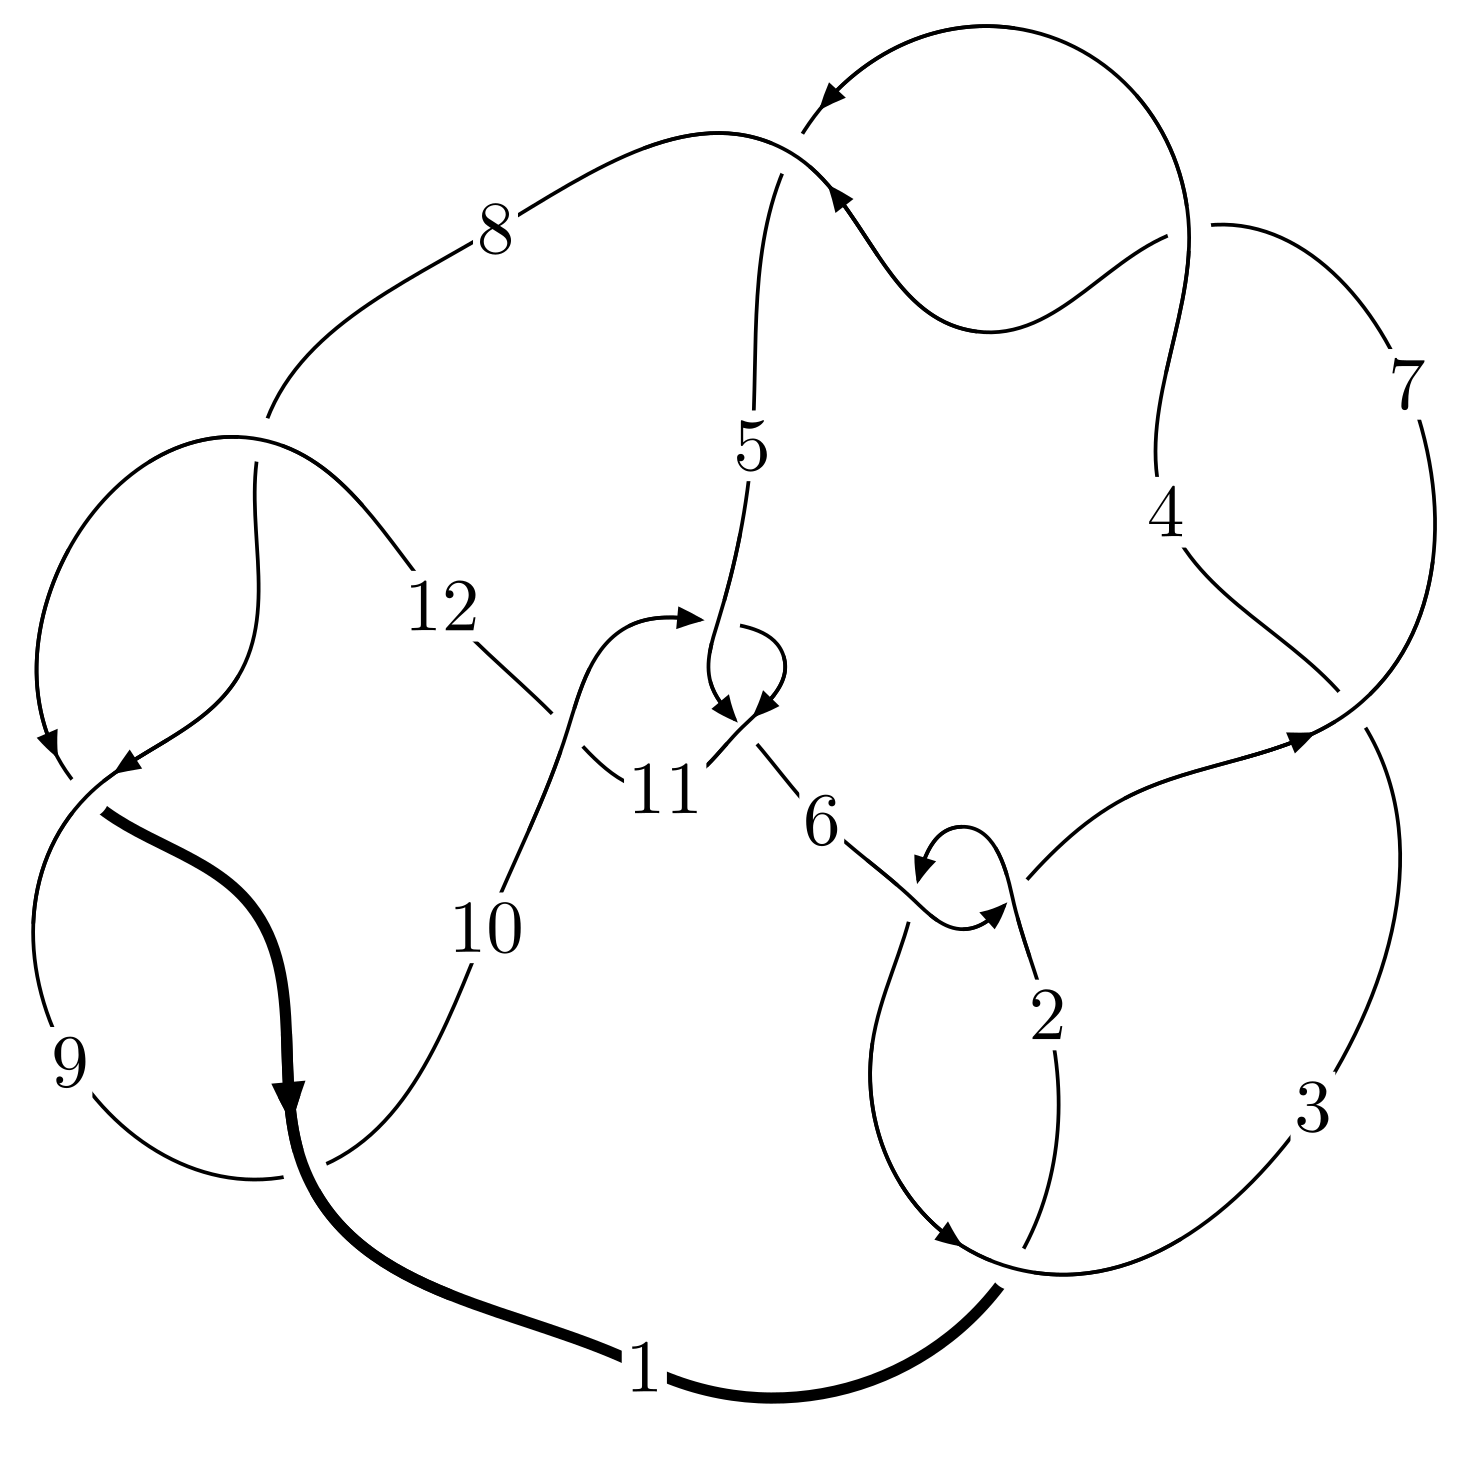
\includegraphics[width=112pt]{../../../GIT/diagram.site/Diagrams/png/1006_12a_0205.png}\\
\ \ \ A knot diagram\footnotemark}&
\allowdisplaybreaks
\textbf{Linearized knot diagam} \\
\cline{2-2}
 &
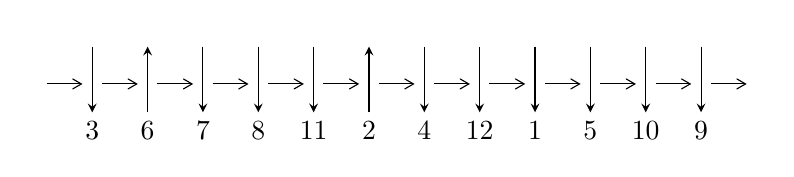
\begin{tikzpicture}[x=20pt, y=17pt]
	% nodes
	\node (C0) at (0, 0) {};
	\node (C1) at (1, 0) {};
	\node (C1U) at (1, +1) {};
	\node (C1D) at (1, -1) {3};

	\node (C2) at (2, 0) {};
	\node (C2U) at (2, +1) {};
	\node (C2D) at (2, -1) {6};

	\node (C3) at (3, 0) {};
	\node (C3U) at (3, +1) {};
	\node (C3D) at (3, -1) {7};

	\node (C4) at (4, 0) {};
	\node (C4U) at (4, +1) {};
	\node (C4D) at (4, -1) {8};

	\node (C5) at (5, 0) {};
	\node (C5U) at (5, +1) {};
	\node (C5D) at (5, -1) {11};

	\node (C6) at (6, 0) {};
	\node (C6U) at (6, +1) {};
	\node (C6D) at (6, -1) {2};

	\node (C7) at (7, 0) {};
	\node (C7U) at (7, +1) {};
	\node (C7D) at (7, -1) {4};

	\node (C8) at (8, 0) {};
	\node (C8U) at (8, +1) {};
	\node (C8D) at (8, -1) {12};

	\node (C9) at (9, 0) {};
	\node (C9U) at (9, +1) {};
	\node (C9D) at (9, -1) {1};

	\node (C10) at (10, 0) {};
	\node (C10U) at (10, +1) {};
	\node (C10D) at (10, -1) {5};

	\node (C11) at (11, 0) {};
	\node (C11U) at (11, +1) {};
	\node (C11D) at (11, -1) {10};

	\node (C12) at (12, 0) {};
	\node (C12U) at (12, +1) {};
	\node (C12D) at (12, -1) {9};
	\node (C13) at (13, 0) {};

	% arrows
	\draw[->,>={angle 60}]
	(C0) edge (C1) (C1) edge (C2) (C2) edge (C3) (C3) edge (C4) (C4) edge (C5) (C5) edge (C6) (C6) edge (C7) (C7) edge (C8) (C8) edge (C9) (C9) edge (C10) (C10) edge (C11) (C11) edge (C12) (C12) edge (C13) ;	\draw[->,>=stealth]
	(C1U) edge (C1D) (C2D) edge (C2U) (C3U) edge (C3D) (C4U) edge (C4D) (C5U) edge (C5D) (C6D) edge (C6U) (C7U) edge (C7D) (C8U) edge (C8D) (C9U) edge (C9D) (C10U) edge (C10D) (C11U) edge (C11D) (C12U) edge (C12D) ;
	\end{tikzpicture} \\
\hhline{~~} \\& 
\textbf{Solving Sequence} \\ \cline{2-2} 
 &
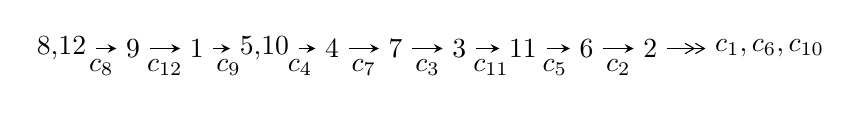
\begin{tikzpicture}[x=23pt, y=7pt]
	% node
	\node (A0) at (-1/8, 0) {8,12};
	\node (A1) at (1, 0) {9};
	\node (A2) at (2, 0) {1};
	\node (A3) at (49/16, 0) {5,10};
	\node (A4) at (33/8, 0) {4};
	\node (A5) at (41/8, 0) {7};
	\node (A6) at (49/8, 0) {3};
	\node (A7) at (57/8, 0) {11};
	\node (A8) at (65/8, 0) {6};
	\node (A9) at (73/8, 0) {2};
	\node (C1) at (1/2, -1) {$c_{8}$};
	\node (C2) at (3/2, -1) {$c_{12}$};
	\node (C3) at (5/2, -1) {$c_{9}$};
	\node (C4) at (29/8, -1) {$c_{4}$};
	\node (C5) at (37/8, -1) {$c_{7}$};
	\node (C6) at (45/8, -1) {$c_{3}$};
	\node (C7) at (53/8, -1) {$c_{11}$};
	\node (C8) at (61/8, -1) {$c_{5}$};
	\node (C9) at (69/8, -1) {$c_{2}$};
	\node (A10) at (11, 0) {$c_{1},c_{6},c_{10}$};

	% edge
	\draw[->,>=stealth]	
	(A0) edge (A1) (A1) edge (A2) (A2) edge (A3) (A3) edge (A4) (A4) edge (A5) (A5) edge (A6) (A6) edge (A7) (A7) edge (A8) (A8) edge (A9) ;
	\draw[->>,>={angle 60}]	
	(A9) edge (A10);
\end{tikzpicture} \\ 

\end{tabular} \\

\footnotetext{
The image of knot diagram is generated by the software ``\textbf{Draw programme}" developed by Andrew Bartholomew(\url{http://www.layer8.co.uk/maths/draw/index.htm\#Running-draw}), where we modified some parts for our purpose(\url{https://github.com/CATsTAILs/LinksPainter}).
}\phantom \\ \newline 
\centering \textbf{Ideals for irreducible components\footnotemark of $X_{\text{par}}$} 
 
\begin{align*}
I^u_{1}&=\langle 
251 u^{73}+1168 u^{72}+\cdots+4 b-189,\;-50 u^{73}-201 u^{72}+\cdots+4 a+23,\;u^{74}+6 u^{73}+\cdots-4 u-1\rangle \\
I^u_{2}&=\langle 
b^5- b^4-2 b^3+b^2+b+1,\;a,\;u-1\rangle \\
\\
\end{align*}
\raggedright * 2 irreducible components of $\dim_{\mathbb{C}}=0$, with total 79 representations.\\
\footnotetext{All coefficients of polynomials are rational numbers. But the coefficients are sometimes approximated in decimal forms when there is not enough margin.}
\newpage
\renewcommand{\arraystretch}{1}
\centering \section*{I. $I^u_{1}= \langle 251 u^{73}+1168 u^{72}+\cdots+4 b-189,\;-50 u^{73}-201 u^{72}+\cdots+4 a+23,\;u^{74}+6 u^{73}+\cdots-4 u-1 \rangle$}
\flushleft \textbf{(i) Arc colorings}\\
\begin{tabular}{m{7pt} m{180pt} m{7pt} m{180pt} }
\flushright $a_{8}=$&$\begin{pmatrix}1\\0\end{pmatrix}$ \\
\flushright $a_{12}=$&$\begin{pmatrix}0\\u\end{pmatrix}$ \\
\flushright $a_{9}=$&$\begin{pmatrix}1\\u^2\end{pmatrix}$ \\
\flushright $a_{1}=$&$\begin{pmatrix}- u\\- u^3+u\end{pmatrix}$ \\
\flushright $a_{5}=$&$\begin{pmatrix}\frac{25}{2} u^{73}+\frac{201}{4} u^{72}+\cdots-\frac{25}{2} u-\frac{23}{4}\\-\frac{251}{4} u^{73}-292 u^{72}+\cdots+\frac{307}{2} u+\frac{189}{4}\end{pmatrix}$ \\
\flushright $a_{10}=$&$\begin{pmatrix}- u^2+1\\- u^4+2 u^2\end{pmatrix}$ \\
\flushright $a_{4}=$&$\begin{pmatrix}-\frac{201}{4} u^{73}-\frac{967}{4} u^{72}+\cdots+141 u+\frac{83}{2}\\-\frac{251}{4} u^{73}-292 u^{72}+\cdots+\frac{307}{2} u+\frac{189}{4}\end{pmatrix}$ \\
\flushright $a_{7}=$&$\begin{pmatrix}0.0625000 u^{73}+0.312500 u^{72}+\cdots-4.18750 u+1.93750\\0.0625000 u^{73}+0.312500 u^{72}+\cdots-1.18750 u-0.0625000\end{pmatrix}$ \\
\flushright $a_{3}=$&$\begin{pmatrix}-30.5625 u^{73}-147.813 u^{72}+\cdots+90.4375 u+26.3125\\30.9375 u^{73}+143.938 u^{72}+\cdots-72.8125 u-22.1875\end{pmatrix}$ \\
\flushright $a_{11}=$&$\begin{pmatrix}u^5-2 u^3+u\\u^7-3 u^5+2 u^3+u\end{pmatrix}$ \\
\flushright $a_{6}=$&$\begin{pmatrix}\frac{25}{2} u^{73}+\frac{269}{4} u^{72}+\cdots-\frac{71}{2} u-\frac{59}{4}\\-\frac{249}{4} u^{73}-\frac{1131}{4} u^{72}+\cdots+141 u+\frac{85}{2}\end{pmatrix}$ \\
\flushright $a_{2}=$&$\begin{pmatrix}-15.1875 u^{73}-73.6875 u^{72}+\cdots+49.3125 u+12.1875\\-19.2500 u^{73}-93.6250 u^{72}+\cdots+54.7500 u+16.8750\end{pmatrix}$\\&\end{tabular}
\flushleft \textbf{(ii) Obstruction class $= -1$}\\~\\
\flushleft \textbf{(iii) Cusp Shapes $= -\frac{177}{4} u^{73}-\frac{1667}{8} u^{72}+\cdots+\frac{477}{4} u+\frac{241}{8}$}\\~\\
\newpage\renewcommand{\arraystretch}{1}
\flushleft \textbf{(iv) u-Polynomials at the component}\newline \\
\begin{tabular}{m{50pt}|m{274pt}}
Crossings & \hspace{64pt}u-Polynomials at each crossing \\
\hline $$\begin{aligned}c_{1}\end{aligned}$$&$\begin{aligned}
&u^{74}+42 u^{73}+\cdots-2 u+1
\end{aligned}$\\
\hline $$\begin{aligned}c_{2},c_{6}\end{aligned}$$&$\begin{aligned}
&u^{74}-2 u^{73}+\cdots-2 u-1
\end{aligned}$\\
\hline $$\begin{aligned}c_{3},c_{4},c_{7}\end{aligned}$$&$\begin{aligned}
&u^{74}+2 u^{73}+\cdots+84 u-17
\end{aligned}$\\
\hline $$\begin{aligned}c_{5},c_{10}\end{aligned}$$&$\begin{aligned}
&u^{74}+u^{73}+\cdots+96 u+32
\end{aligned}$\\
\hline $$\begin{aligned}c_{8},c_{9},c_{12}\end{aligned}$$&$\begin{aligned}
&u^{74}-6 u^{73}+\cdots+4 u-1
\end{aligned}$\\
\hline $$\begin{aligned}c_{11}\end{aligned}$$&$\begin{aligned}
&u^{74}+33 u^{73}+\cdots+7680 u+1024
\end{aligned}$\\
\hline
\end{tabular}\\~\\
\newpage\renewcommand{\arraystretch}{1}
\flushleft \textbf{(v) Riley Polynomials at the component}\newline \\
\begin{tabular}{m{50pt}|m{274pt}}
Crossings & \hspace{64pt}Riley Polynomials at each crossing \\
\hline $$\begin{aligned}c_{1}\end{aligned}$$&$\begin{aligned}
&y^{74}-18 y^{73}+\cdots-70 y+1
\end{aligned}$\\
\hline $$\begin{aligned}c_{2},c_{6}\end{aligned}$$&$\begin{aligned}
&y^{74}+42 y^{73}+\cdots-2 y+1
\end{aligned}$\\
\hline $$\begin{aligned}c_{3},c_{4},c_{7}\end{aligned}$$&$\begin{aligned}
&y^{74}-78 y^{73}+\cdots-14298 y+289
\end{aligned}$\\
\hline $$\begin{aligned}c_{5},c_{10}\end{aligned}$$&$\begin{aligned}
&y^{74}-33 y^{73}+\cdots-7680 y+1024
\end{aligned}$\\
\hline $$\begin{aligned}c_{8},c_{9},c_{12}\end{aligned}$$&$\begin{aligned}
&y^{74}-66 y^{73}+\cdots-4 y+1
\end{aligned}$\\
\hline $$\begin{aligned}c_{11}\end{aligned}$$&$\begin{aligned}
&y^{74}+7 y^{73}+\cdots-12189696 y+1048576
\end{aligned}$\\
\hline
\end{tabular}\\~\\
\newpage\flushleft \textbf{(vi) Complex Volumes and Cusp Shapes}
$$\begin{array}{c|c|c}  
\text{Solutions to }I^u_{1}& \I (\text{vol} + \sqrt{-1}CS) & \text{Cusp shape}\\
 \hline 
\begin{aligned}
u &= \phantom{-}0.881128 + 0.574262 I \\
a &= -0.392145 - 0.461104 I \\
b &= \phantom{-}1.51995 + 0.06899 I\end{aligned}
 & -10.03960 - 3.52098 I & \phantom{-0.000000 } 0 \\ \hline\begin{aligned}
u &= \phantom{-}0.881128 - 0.574262 I \\
a &= -0.392145 + 0.461104 I \\
b &= \phantom{-}1.51995 - 0.06899 I\end{aligned}
 & -10.03960 + 3.52098 I & \phantom{-0.000000 } 0 \\ \hline\begin{aligned}
u &= \phantom{-}0.988283 + 0.362341 I \\
a &= \phantom{-}0.732096 - 0.013015 I \\
b &= -0.662384 + 0.595002 I\end{aligned}
 & -2.23570 + 2.76072 I & \phantom{-0.000000 } 0 \\ \hline\begin{aligned}
u &= \phantom{-}0.988283 - 0.362341 I \\
a &= \phantom{-}0.732096 + 0.013015 I \\
b &= -0.662384 - 0.595002 I\end{aligned}
 & -2.23570 - 2.76072 I & \phantom{-0.000000 } 0 \\ \hline\begin{aligned}
u &= \phantom{-}0.900199 + 0.549025 I \\
a &= \phantom{-}0.478227 + 0.417353 I \\
b &= -1.45382 + 0.10364 I\end{aligned}
 & -6.21271 + 1.04580 I & \phantom{-0.000000 } 0 \\ \hline\begin{aligned}
u &= \phantom{-}0.900199 - 0.549025 I \\
a &= \phantom{-}0.478227 - 0.417353 I \\
b &= -1.45382 - 0.10364 I\end{aligned}
 & -6.21271 - 1.04580 I & \phantom{-0.000000 } 0 \\ \hline\begin{aligned}
u &= \phantom{-}0.925360 + 0.561900 I \\
a &= -0.535816 - 0.483396 I \\
b &= \phantom{-}1.59118 - 0.20476 I\end{aligned}
 & -9.79897 + 5.80428 I & \phantom{-0.000000 } 0 \\ \hline\begin{aligned}
u &= \phantom{-}0.925360 - 0.561900 I \\
a &= -0.535816 + 0.483396 I \\
b &= \phantom{-}1.59118 + 0.20476 I\end{aligned}
 & -9.79897 - 5.80428 I & \phantom{-0.000000 } 0 \\ \hline\begin{aligned}
u &= \phantom{-}0.287137 + 0.859379 I \\
a &= -1.13110 - 1.36816 I \\
b &= \phantom{-}1.62687 + 0.25833 I\end{aligned}
 & -7.84795 - 10.78640 I & \phantom{-0.000000 } 0 \\ \hline\begin{aligned}
u &= \phantom{-}0.287137 - 0.859379 I \\
a &= -1.13110 + 1.36816 I \\
b &= \phantom{-}1.62687 - 0.25833 I\end{aligned}
 & -7.84795 + 10.78640 I & \phantom{-0.000000 } 0\\
 \hline 
 \end{array}$$\newpage$$\begin{array}{c|c|c}  
\text{Solutions to }I^u_{1}& \I (\text{vol} + \sqrt{-1}CS) & \text{Cusp shape}\\
 \hline 
\begin{aligned}
u &= \phantom{-}0.314792 + 0.842150 I \\
a &= -1.08527 - 1.22153 I \\
b &= \phantom{-}1.48731 + 0.00206 I\end{aligned}
 & -8.30896 - 1.43299 I & \phantom{-0.000000 } 0 \\ \hline\begin{aligned}
u &= \phantom{-}0.314792 - 0.842150 I \\
a &= -1.08527 + 1.22153 I \\
b &= \phantom{-}1.48731 - 0.00206 I\end{aligned}
 & -8.30896 + 1.43299 I & \phantom{-0.000000 } 0 \\ \hline\begin{aligned}
u &= \phantom{-}0.292088 + 0.841513 I \\
a &= \phantom{-}1.05644 + 1.32316 I \\
b &= -1.47219 - 0.19833 I\end{aligned}
 & -4.34649 - 5.92708 I & \phantom{-0.000000 } 0 \\ \hline\begin{aligned}
u &= \phantom{-}0.292088 - 0.841513 I \\
a &= \phantom{-}1.05644 - 1.32316 I \\
b &= -1.47219 + 0.19833 I\end{aligned}
 & -4.34649 + 5.92708 I & \phantom{-0.000000 } 0 \\ \hline\begin{aligned}
u &= \phantom{-}1.085780 + 0.243540 I \\
a &= -0.729453 + 0.365525 I \\
b &= \phantom{-}0.124325 - 0.592140 I\end{aligned}
 & -0.968890 - 0.789801 I & \phantom{-0.000000 } 0 \\ \hline\begin{aligned}
u &= \phantom{-}1.085780 - 0.243540 I \\
a &= -0.729453 - 0.365525 I \\
b &= \phantom{-}0.124325 + 0.592140 I\end{aligned}
 & -0.968890 + 0.789801 I & \phantom{-0.000000 } 0 \\ \hline\begin{aligned}
u &= \phantom{-}0.201797 + 0.773580 I \\
a &= \phantom{-}0.65000 + 1.60035 I \\
b &= -0.793170 - 0.734810 I\end{aligned}
 & \phantom{-}0.15931 - 6.92492 I & -8.00000 + 9.41570 I \\ \hline\begin{aligned}
u &= \phantom{-}0.201797 - 0.773580 I \\
a &= \phantom{-}0.65000 - 1.60035 I \\
b &= -0.793170 + 0.734810 I\end{aligned}
 & \phantom{-}0.15931 + 6.92492 I & -8.00000 - 9.41570 I \\ \hline\begin{aligned}
u &= \phantom{-}1.203160 + 0.212321 I \\
a &= -0.835102 + 0.755842 I \\
b &= -0.352089 - 0.569580 I\end{aligned}
 & -1.26241 - 1.26238 I & \phantom{-0.000000 } 0 \\ \hline\begin{aligned}
u &= \phantom{-}1.203160 - 0.212321 I \\
a &= -0.835102 - 0.755842 I \\
b &= -0.352089 + 0.569580 I\end{aligned}
 & -1.26241 + 1.26238 I & \phantom{-0.000000 } 0\\
 \hline 
 \end{array}$$\newpage$$\begin{array}{c|c|c}  
\text{Solutions to }I^u_{1}& \I (\text{vol} + \sqrt{-1}CS) & \text{Cusp shape}\\
 \hline 
\begin{aligned}
u &= \phantom{-}0.636386 + 0.433353 I \\
a &= \phantom{-}0.248415 - 0.156107 I \\
b &= -0.539496 - 0.235219 I\end{aligned}
 & -3.20093 - 2.38936 I & -17.3308 + 5.2603 I \\ \hline\begin{aligned}
u &= \phantom{-}0.636386 - 0.433353 I \\
a &= \phantom{-}0.248415 + 0.156107 I \\
b &= -0.539496 + 0.235219 I\end{aligned}
 & -3.20093 + 2.38936 I & -17.3308 - 5.2603 I \\ \hline\begin{aligned}
u &= \phantom{-}0.174212 + 0.714774 I \\
a &= -0.39734 - 1.61036 I \\
b &= \phantom{-}0.393692 + 0.706879 I\end{aligned}
 & \phantom{-}1.68253 - 2.79181 I & -4.40821 + 4.21273 I \\ \hline\begin{aligned}
u &= \phantom{-}0.174212 - 0.714774 I \\
a &= -0.39734 + 1.61036 I \\
b &= \phantom{-}0.393692 - 0.706879 I\end{aligned}
 & \phantom{-}1.68253 + 2.79181 I & -4.40821 - 4.21273 I \\ \hline\begin{aligned}
u &= \phantom{-}0.319686 + 0.646062 I \\
a &= \phantom{-}0.316719 + 1.035180 I \\
b &= -0.300560 + 0.024775 I\end{aligned}
 & -2.20621 - 1.45129 I & -14.5147 + 3.3145 I \\ \hline\begin{aligned}
u &= \phantom{-}0.319686 - 0.646062 I \\
a &= \phantom{-}0.316719 - 1.035180 I \\
b &= -0.300560 - 0.024775 I\end{aligned}
 & -2.20621 + 1.45129 I & -14.5147 - 3.3145 I \\ \hline\begin{aligned}
u &= \phantom{-}1.285420 + 0.094016 I \\
a &= \phantom{-}0.456290 - 1.265580 I \\
b &= \phantom{-}0.430143 - 0.102358 I\end{aligned}
 & -4.61992 + 0.36511 I & \phantom{-0.000000 } 0 \\ \hline\begin{aligned}
u &= \phantom{-}1.285420 - 0.094016 I \\
a &= \phantom{-}0.456290 + 1.265580 I \\
b &= \phantom{-}0.430143 + 0.102358 I\end{aligned}
 & -4.61992 - 0.36511 I & \phantom{-0.000000 } 0 \\ \hline\begin{aligned}
u &= -1.287860 + 0.072895 I \\
a &= \phantom{-}0.147765 + 0.194840 I \\
b &= -1.36565 - 0.38952 I\end{aligned}
 & -8.72493 - 4.01377 I & \phantom{-0.000000 } 0 \\ \hline\begin{aligned}
u &= -1.287860 - 0.072895 I \\
a &= \phantom{-}0.147765 - 0.194840 I \\
b &= -1.36565 + 0.38952 I\end{aligned}
 & -8.72493 + 4.01377 I & \phantom{-0.000000 } 0\\
 \hline 
 \end{array}$$\newpage$$\begin{array}{c|c|c}  
\text{Solutions to }I^u_{1}& \I (\text{vol} + \sqrt{-1}CS) & \text{Cusp shape}\\
 \hline 
\begin{aligned}
u &= \phantom{-}1.273630 + 0.234512 I \\
a &= \phantom{-}1.06836 - 0.97934 I \\
b &= \phantom{-}0.772121 + 0.649670 I\end{aligned}
 & -2.86722 - 5.13648 I & \phantom{-0.000000 } 0 \\ \hline\begin{aligned}
u &= \phantom{-}1.273630 - 0.234512 I \\
a &= \phantom{-}1.06836 + 0.97934 I \\
b &= \phantom{-}0.772121 - 0.649670 I\end{aligned}
 & -2.86722 + 5.13648 I & \phantom{-0.000000 } 0 \\ \hline\begin{aligned}
u &= -1.310770 + 0.210855 I \\
a &= -0.365749 - 0.628451 I \\
b &= \phantom{-}0.464829 + 0.924450 I\end{aligned}
 & -3.02836 + 0.78893 I & \phantom{-0.000000 } 0 \\ \hline\begin{aligned}
u &= -1.310770 - 0.210855 I \\
a &= -0.365749 + 0.628451 I \\
b &= \phantom{-}0.464829 - 0.924450 I\end{aligned}
 & -3.02836 - 0.78893 I & \phantom{-0.000000 } 0 \\ \hline\begin{aligned}
u &= -1.327870 + 0.109441 I \\
a &= -0.078373 - 0.356478 I \\
b &= \phantom{-}1.041460 + 0.386661 I\end{aligned}
 & -5.77899 + 0.48003 I & \phantom{-0.000000 } 0 \\ \hline\begin{aligned}
u &= -1.327870 - 0.109441 I \\
a &= -0.078373 + 0.356478 I \\
b &= \phantom{-}1.041460 - 0.386661 I\end{aligned}
 & -5.77899 - 0.48003 I & \phantom{-0.000000 } 0 \\ \hline\begin{aligned}
u &= \phantom{-}0.090587 + 0.645600 I \\
a &= -0.05614 - 1.76780 I \\
b &= -0.143845 + 0.767387 I\end{aligned}
 & \phantom{-}2.07073 - 1.86749 I & -2.85319 + 4.16997 I \\ \hline\begin{aligned}
u &= \phantom{-}0.090587 - 0.645600 I \\
a &= -0.05614 + 1.76780 I \\
b &= -0.143845 - 0.767387 I\end{aligned}
 & \phantom{-}2.07073 + 1.86749 I & -2.85319 - 4.16997 I \\ \hline\begin{aligned}
u &= -1.331220 + 0.247307 I \\
a &= \phantom{-}0.423310 + 0.804300 I \\
b &= -0.061462 - 0.941261 I\end{aligned}
 & -2.41235 + 5.09301 I & \phantom{-0.000000 } 0 \\ \hline\begin{aligned}
u &= -1.331220 - 0.247307 I \\
a &= \phantom{-}0.423310 - 0.804300 I \\
b &= -0.061462 + 0.941261 I\end{aligned}
 & -2.41235 - 5.09301 I & \phantom{-0.000000 } 0\\
 \hline 
 \end{array}$$\newpage$$\begin{array}{c|c|c}  
\text{Solutions to }I^u_{1}& \I (\text{vol} + \sqrt{-1}CS) & \text{Cusp shape}\\
 \hline 
\begin{aligned}
u &= \phantom{-}1.372500 + 0.208067 I \\
a &= \phantom{-}1.18530 - 1.51605 I \\
b &= \phantom{-}1.47714 + 0.15260 I\end{aligned}
 & -7.28647 - 3.73730 I & \phantom{-0.000000 } 0 \\ \hline\begin{aligned}
u &= \phantom{-}1.372500 - 0.208067 I \\
a &= \phantom{-}1.18530 + 1.51605 I \\
b &= \phantom{-}1.47714 - 0.15260 I\end{aligned}
 & -7.28647 + 3.73730 I & \phantom{-0.000000 } 0 \\ \hline\begin{aligned}
u &= \phantom{-}1.384380 + 0.195037 I \\
a &= -1.14266 + 1.61351 I \\
b &= -1.51278 + 0.02690 I\end{aligned}
 & -11.19560 + 0.80901 I & \phantom{-0.000000 } 0 \\ \hline\begin{aligned}
u &= \phantom{-}1.384380 - 0.195037 I \\
a &= -1.14266 - 1.61351 I \\
b &= -1.51278 - 0.02690 I\end{aligned}
 & -11.19560 - 0.80901 I & \phantom{-0.000000 } 0 \\ \hline\begin{aligned}
u &= -1.368220 + 0.287711 I \\
a &= \phantom{-}0.456831 + 1.079290 I \\
b &= \phantom{-}0.530276 - 0.801232 I\end{aligned}
 & -3.20875 + 6.42514 I & \phantom{-0.000000 } 0 \\ \hline\begin{aligned}
u &= -1.368220 - 0.287711 I \\
a &= \phantom{-}0.456831 - 1.079290 I \\
b &= \phantom{-}0.530276 + 0.801232 I\end{aligned}
 & -3.20875 - 6.42514 I & \phantom{-0.000000 } 0 \\ \hline\begin{aligned}
u &= \phantom{-}0.001762 + 0.601615 I \\
a &= -0.18960 + 1.93159 I \\
b &= \phantom{-}0.582995 - 0.743414 I\end{aligned}
 & \phantom{-}1.09588 + 2.08440 I & -5.27577 - 3.44831 I \\ \hline\begin{aligned}
u &= \phantom{-}0.001762 - 0.601615 I \\
a &= -0.18960 - 1.93159 I \\
b &= \phantom{-}0.582995 + 0.743414 I\end{aligned}
 & \phantom{-}1.09588 - 2.08440 I & -5.27577 + 3.44831 I \\ \hline\begin{aligned}
u &= \phantom{-}1.381070 + 0.220674 I \\
a &= -1.27621 + 1.52980 I \\
b &= -1.61885 - 0.22827 I\end{aligned}
 & -10.84100 - 8.56310 I & \phantom{-0.000000 } 0 \\ \hline\begin{aligned}
u &= \phantom{-}1.381070 - 0.220674 I \\
a &= -1.27621 - 1.52980 I \\
b &= -1.61885 + 0.22827 I\end{aligned}
 & -10.84100 + 8.56310 I & \phantom{-0.000000 } 0\\
 \hline 
 \end{array}$$\newpage$$\begin{array}{c|c|c}  
\text{Solutions to }I^u_{1}& \I (\text{vol} + \sqrt{-1}CS) & \text{Cusp shape}\\
 \hline 
\begin{aligned}
u &= -1.406650 + 0.108118 I \\
a &= -0.224298 + 0.479931 I \\
b &= -0.889838 + 0.012840 I\end{aligned}
 & -9.56584 + 3.88184 I & \phantom{-0.000000 } 0 \\ \hline\begin{aligned}
u &= -1.406650 - 0.108118 I \\
a &= -0.224298 - 0.479931 I \\
b &= -0.889838 - 0.012840 I\end{aligned}
 & -9.56584 - 3.88184 I & \phantom{-0.000000 } 0 \\ \hline\begin{aligned}
u &= -1.38177 + 0.31309 I \\
a &= -0.519776 - 1.227890 I \\
b &= -0.894583 + 0.801624 I\end{aligned}
 & -4.86125 + 10.84660 I & \phantom{-0.000000 } 0 \\ \hline\begin{aligned}
u &= -1.38177 - 0.31309 I \\
a &= -0.519776 + 1.227890 I \\
b &= -0.894583 - 0.801624 I\end{aligned}
 & -4.86125 - 10.84660 I & \phantom{-0.000000 } 0 \\ \hline\begin{aligned}
u &= -0.217146 + 0.536055 I \\
a &= \phantom{-}0.60175 - 2.16828 I \\
b &= -1.52812 + 0.24824 I\end{aligned}
 & -5.74382 + 5.73352 I & -9.31960 - 3.96496 I \\ \hline\begin{aligned}
u &= -0.217146 - 0.536055 I \\
a &= \phantom{-}0.60175 + 2.16828 I \\
b &= -1.52812 - 0.24824 I\end{aligned}
 & -5.74382 - 5.73352 I & -9.31960 + 3.96496 I \\ \hline\begin{aligned}
u &= -1.40915 + 0.25179 I \\
a &= -0.157565 - 1.105170 I \\
b &= -0.323961 + 0.190846 I\end{aligned}
 & -7.68685 + 4.72210 I & \phantom{-0.000000 } 0 \\ \hline\begin{aligned}
u &= -1.40915 - 0.25179 I \\
a &= -0.157565 + 1.105170 I \\
b &= -0.323961 - 0.190846 I\end{aligned}
 & -7.68685 - 4.72210 I & \phantom{-0.000000 } 0 \\ \hline\begin{aligned}
u &= -0.195506 + 0.494386 I \\
a &= -0.60346 + 2.10373 I \\
b &= \phantom{-}1.332360 - 0.127865 I\end{aligned}
 & -2.28691 + 1.08117 I & -6.04411 - 0.68667 I \\ \hline\begin{aligned}
u &= -0.195506 - 0.494386 I \\
a &= -0.60346 - 2.10373 I \\
b &= \phantom{-}1.332360 + 0.127865 I\end{aligned}
 & -2.28691 - 1.08117 I & -6.04411 + 0.68667 I\\
 \hline 
 \end{array}$$\newpage$$\begin{array}{c|c|c}  
\text{Solutions to }I^u_{1}& \I (\text{vol} + \sqrt{-1}CS) & \text{Cusp shape}\\
 \hline 
\begin{aligned}
u &= -1.43492 + 0.33574 I \\
a &= -0.42182 - 1.57242 I \\
b &= -1.52280 + 0.24815 I\end{aligned}
 & -9.8574 + 10.1740 I & \phantom{-0.000000 } 0 \\ \hline\begin{aligned}
u &= -1.43492 - 0.33574 I \\
a &= -0.42182 + 1.57242 I \\
b &= -1.52280 - 0.24815 I\end{aligned}
 & -9.8574 - 10.1740 I & \phantom{-0.000000 } 0 \\ \hline\begin{aligned}
u &= -0.244545 + 0.465151 I \\
a &= \phantom{-}0.66363 - 2.09922 I \\
b &= -1.43543 - 0.11457 I\end{aligned}
 & -6.00989 - 3.31774 I & -9.52284 + 2.54149 I \\ \hline\begin{aligned}
u &= -0.244545 - 0.465151 I \\
a &= \phantom{-}0.66363 + 2.09922 I \\
b &= -1.43543 + 0.11457 I\end{aligned}
 & -6.00989 + 3.31774 I & -9.52284 - 2.54149 I \\ \hline\begin{aligned}
u &= -1.43676 + 0.34496 I \\
a &= \phantom{-}0.46165 + 1.62078 I \\
b &= \phantom{-}1.67048 - 0.27980 I\end{aligned}
 & -13.3475 + 15.1287 I & \phantom{-0.000000 } 0 \\ \hline\begin{aligned}
u &= -1.43676 - 0.34496 I \\
a &= \phantom{-}0.46165 - 1.62078 I \\
b &= \phantom{-}1.67048 + 0.27980 I\end{aligned}
 & -13.3475 - 15.1287 I & \phantom{-0.000000 } 0 \\ \hline\begin{aligned}
u &= -1.44511 + 0.33011 I \\
a &= \phantom{-}0.34935 + 1.59979 I \\
b &= \phantom{-}1.49951 - 0.06456 I\end{aligned}
 & -13.9374 + 5.6612 I & \phantom{-0.000000 } 0 \\ \hline\begin{aligned}
u &= -1.44511 - 0.33011 I \\
a &= \phantom{-}0.34935 - 1.59979 I \\
b &= \phantom{-}1.49951 + 0.06456 I\end{aligned}
 & -13.9374 - 5.6612 I & \phantom{-0.000000 } 0 \\ \hline\begin{aligned}
u &= -1.52087\phantom{ +0.000000I} \\
a &= -0.926353\phantom{ +0.000000I} \\
b &= -1.58708\phantom{ +0.000000I}\end{aligned}
 & -14.6359\phantom{ +0.000000I} & \phantom{-0.000000 } 0 \\ \hline\begin{aligned}
u &= -1.52946 + 0.01186 I \\
a &= \phantom{-}0.979765 - 0.076295 I \\
b &= \phantom{-}1.64505 - 0.09028 I\end{aligned}
 & -18.4592 + 4.8158 I & \phantom{-0.000000 } 0\\
 \hline 
 \end{array}$$\newpage$$\begin{array}{c|c|c}  
\text{Solutions to }I^u_{1}& \I (\text{vol} + \sqrt{-1}CS) & \text{Cusp shape}\\
 \hline 
\begin{aligned}
u &= -1.52946 - 0.01186 I \\
a &= \phantom{-}0.979765 + 0.076295 I \\
b &= \phantom{-}1.64505 + 0.09028 I\end{aligned}
 & -18.4592 - 4.8158 I & \phantom{-0.000000 } 0 \\ \hline\begin{aligned}
u &= \phantom{-}0.438993\phantom{ +0.000000I} \\
a &= -0.875494\phantom{ +0.000000I} \\
b &= \phantom{-}0.359702\phantom{ +0.000000I}\end{aligned}
 & -0.831134\phantom{ +0.000000I} & -11.9340\phantom{ +0.000000I} \\ \hline\begin{aligned}
u &= -0.131466 + 0.110386 I \\
a &= -0.73310 + 2.64270 I \\
b &= \phantom{-}0.295035 + 0.455623 I\end{aligned}
 & -0.50060 - 1.35724 I & -5.01014 + 4.53923 I \\ \hline\begin{aligned}
u &= -0.131466 - 0.110386 I \\
a &= -0.73310 - 2.64270 I \\
b &= \phantom{-}0.295035 - 0.455623 I\end{aligned}
 & -0.50060 + 1.35724 I & -5.01014 - 4.53923 I\\
 \hline 
 \end{array}$$\newpage\newpage\renewcommand{\arraystretch}{1}
\centering \section*{II. $I^u_{2}= \langle b^5- b^4-2 b^3+b^2+b+1,\;a,\;u-1 \rangle$}
\flushleft \textbf{(i) Arc colorings}\\
\begin{tabular}{m{7pt} m{180pt} m{7pt} m{180pt} }
\flushright $a_{8}=$&$\begin{pmatrix}1\\0\end{pmatrix}$ \\
\flushright $a_{12}=$&$\begin{pmatrix}0\\1\end{pmatrix}$ \\
\flushright $a_{9}=$&$\begin{pmatrix}1\\1\end{pmatrix}$ \\
\flushright $a_{1}=$&$\begin{pmatrix}-1\\0\end{pmatrix}$ \\
\flushright $a_{5}=$&$\begin{pmatrix}0\\b\end{pmatrix}$ \\
\flushright $a_{10}=$&$\begin{pmatrix}0\\1\end{pmatrix}$ \\
\flushright $a_{4}=$&$\begin{pmatrix}b\\b\end{pmatrix}$ \\
\flushright $a_{7}=$&$\begin{pmatrix}- b^2+1\\- b^2\end{pmatrix}$ \\
\flushright $a_{3}=$&$\begin{pmatrix}- b^3+2 b\\- b^3+b\end{pmatrix}$ \\
\flushright $a_{11}=$&$\begin{pmatrix}0\\1\end{pmatrix}$ \\
\flushright $a_{6}=$&$\begin{pmatrix}0\\b\end{pmatrix}$ \\
\flushright $a_{2}=$&$\begin{pmatrix}- b^3+2 b\\- b^4- b^3+b^2+2 b+1\end{pmatrix}$\\&\end{tabular}
\flushleft \textbf{(ii) Obstruction class $= 1$}\\~\\
\flushleft \textbf{(iii) Cusp Shapes $= b^4+2 b^3-5 b-14$}\\~\\
\newpage\renewcommand{\arraystretch}{1}
\flushleft \textbf{(iv) u-Polynomials at the component}\newline \\
\begin{tabular}{m{50pt}|m{274pt}}
Crossings & \hspace{64pt}u-Polynomials at each crossing \\
\hline $$\begin{aligned}c_{1}\end{aligned}$$&$\begin{aligned}
&u^5-3 u^4+4 u^3- u^2- u+1
\end{aligned}$\\
\hline $$\begin{aligned}c_{2}\end{aligned}$$&$\begin{aligned}
&u^5- u^4+2 u^3- u^2+u-1
\end{aligned}$\\
\hline $$\begin{aligned}c_{3},c_{4}\end{aligned}$$&$\begin{aligned}
&u^5+u^4-2 u^3- u^2+u-1
\end{aligned}$\\
\hline $$\begin{aligned}c_{5},c_{10},c_{11}\end{aligned}$$&$\begin{aligned}
&u^5
\end{aligned}$\\
\hline $$\begin{aligned}c_{6}\end{aligned}$$&$\begin{aligned}
&u^5+u^4+2 u^3+u^2+u+1
\end{aligned}$\\
\hline $$\begin{aligned}c_{7}\end{aligned}$$&$\begin{aligned}
&u^5- u^4-2 u^3+u^2+u+1
\end{aligned}$\\
\hline $$\begin{aligned}c_{8},c_{9}\end{aligned}$$&$\begin{aligned}
&(u-1)^5
\end{aligned}$\\
\hline $$\begin{aligned}c_{12}\end{aligned}$$&$\begin{aligned}
&(u+1)^5
\end{aligned}$\\
\hline
\end{tabular}\\~\\
\newpage\renewcommand{\arraystretch}{1}
\flushleft \textbf{(v) Riley Polynomials at the component}\newline \\
\begin{tabular}{m{50pt}|m{274pt}}
Crossings & \hspace{64pt}Riley Polynomials at each crossing \\
\hline $$\begin{aligned}c_{1}\end{aligned}$$&$\begin{aligned}
&y^5- y^4+8 y^3-3 y^2+3 y-1
\end{aligned}$\\
\hline $$\begin{aligned}c_{2},c_{6}\end{aligned}$$&$\begin{aligned}
&y^5+3 y^4+4 y^3+y^2- y-1
\end{aligned}$\\
\hline $$\begin{aligned}c_{3},c_{4},c_{7}\end{aligned}$$&$\begin{aligned}
&y^5-5 y^4+8 y^3-3 y^2- y-1
\end{aligned}$\\
\hline $$\begin{aligned}c_{5},c_{10},c_{11}\end{aligned}$$&$\begin{aligned}
&y^5
\end{aligned}$\\
\hline $$\begin{aligned}c_{8},c_{9},c_{12}\end{aligned}$$&$\begin{aligned}
&(y-1)^5
\end{aligned}$\\
\hline
\end{tabular}\\~\\
\newpage\flushleft \textbf{(vi) Complex Volumes and Cusp Shapes}
$$\begin{array}{c|c|c}  
\text{Solutions to }I^u_{2}& \I (\text{vol} + \sqrt{-1}CS) & \text{Cusp shape}\\
 \hline 
\begin{aligned}
u &= \phantom{-}1.00000\phantom{ +0.000000I} \\
a &= \phantom{-0.000000 } 0 \\
b &= -1.21774\phantom{ +0.000000I}\end{aligned}
 & -4.04602\phantom{ +0.000000I} & -9.32390\phantom{ +0.000000I} \\ \hline\begin{aligned}
u &= \phantom{-}1.00000\phantom{ +0.000000I} \\
a &= \phantom{-0.000000 } 0 \\
b &= -0.309916 + 0.549911 I\end{aligned}
 & -1.97403 + 1.53058 I & -12.02124 - 2.62456 I \\ \hline\begin{aligned}
u &= \phantom{-}1.00000\phantom{ +0.000000I} \\
a &= \phantom{-0.000000 } 0 \\
b &= -0.309916 - 0.549911 I\end{aligned}
 & -1.97403 - 1.53058 I & -12.02124 + 2.62456 I \\ \hline\begin{aligned}
u &= \phantom{-}1.00000\phantom{ +0.000000I} \\
a &= \phantom{-0.000000 } 0 \\
b &= \phantom{-}1.41878 + 0.21917 I\end{aligned}
 & -7.51750 - 4.40083 I & -12.31681 + 3.97407 I \\ \hline\begin{aligned}
u &= \phantom{-}1.00000\phantom{ +0.000000I} \\
a &= \phantom{-0.000000 } 0 \\
b &= \phantom{-}1.41878 - 0.21917 I\end{aligned}
 & -7.51750 + 4.40083 I & -12.31681 - 3.97407 I\\
 \hline 
 \end{array}$$\newpage
\newpage\renewcommand{\arraystretch}{1}
\centering \section*{ III. u-Polynomials}
\begin{tabular}{m{50pt}|m{274pt}}
Crossings & \hspace{64pt}u-Polynomials at each crossing \\
\hline $$\begin{aligned}c_{1}\end{aligned}$$&$\begin{aligned}
&(u^5-3 u^4+4 u^3- u^2- u+1)(u^{74}+42 u^{73}+\cdots-2 u+1)
\end{aligned}$\\
\hline $$\begin{aligned}c_{2}\end{aligned}$$&$\begin{aligned}
&(u^5- u^4+2 u^3- u^2+u-1)(u^{74}-2 u^{73}+\cdots-2 u-1)
\end{aligned}$\\
\hline $$\begin{aligned}c_{3},c_{4}\end{aligned}$$&$\begin{aligned}
&(u^5+u^4-2 u^3- u^2+u-1)(u^{74}+2 u^{73}+\cdots+84 u-17)
\end{aligned}$\\
\hline $$\begin{aligned}c_{5},c_{10}\end{aligned}$$&$\begin{aligned}
&u^5(u^{74}+u^{73}+\cdots+96 u+32)
\end{aligned}$\\
\hline $$\begin{aligned}c_{6}\end{aligned}$$&$\begin{aligned}
&(u^5+u^4+2 u^3+u^2+u+1)(u^{74}-2 u^{73}+\cdots-2 u-1)
\end{aligned}$\\
\hline $$\begin{aligned}c_{7}\end{aligned}$$&$\begin{aligned}
&(u^5- u^4-2 u^3+u^2+u+1)(u^{74}+2 u^{73}+\cdots+84 u-17)
\end{aligned}$\\
\hline $$\begin{aligned}c_{8},c_{9}\end{aligned}$$&$\begin{aligned}
&((u-1)^5)(u^{74}-6 u^{73}+\cdots+4 u-1)
\end{aligned}$\\
\hline $$\begin{aligned}c_{11}\end{aligned}$$&$\begin{aligned}
&u^5(u^{74}+33 u^{73}+\cdots+7680 u+1024)
\end{aligned}$\\
\hline $$\begin{aligned}c_{12}\end{aligned}$$&$\begin{aligned}
&((u+1)^5)(u^{74}-6 u^{73}+\cdots+4 u-1)
\end{aligned}$\\
\hline
\end{tabular}\newpage\renewcommand{\arraystretch}{1}
\centering \section*{ IV. Riley Polynomials}
\begin{tabular}{m{50pt}|m{274pt}}
Crossings & \hspace{64pt}Riley Polynomials at each crossing \\
\hline $$\begin{aligned}c_{1}\end{aligned}$$&$\begin{aligned}
&(y^5- y^4+8 y^3-3 y^2+3 y-1)(y^{74}-18 y^{73}+\cdots-70 y+1)
\end{aligned}$\\
\hline $$\begin{aligned}c_{2},c_{6}\end{aligned}$$&$\begin{aligned}
&(y^5+3 y^4+4 y^3+y^2- y-1)(y^{74}+42 y^{73}+\cdots-2 y+1)
\end{aligned}$\\
\hline $$\begin{aligned}c_{3},c_{4},c_{7}\end{aligned}$$&$\begin{aligned}
&(y^5-5 y^4+8 y^3-3 y^2- y-1)(y^{74}-78 y^{73}+\cdots-14298 y+289)
\end{aligned}$\\
\hline $$\begin{aligned}c_{5},c_{10}\end{aligned}$$&$\begin{aligned}
&y^5(y^{74}-33 y^{73}+\cdots-7680 y+1024)
\end{aligned}$\\
\hline $$\begin{aligned}c_{8},c_{9},c_{12}\end{aligned}$$&$\begin{aligned}
&((y-1)^5)(y^{74}-66 y^{73}+\cdots-4 y+1)
\end{aligned}$\\
\hline $$\begin{aligned}c_{11}\end{aligned}$$&$\begin{aligned}
&y^5(y^{74}+7 y^{73}+\cdots-1.21897\times10^{7} y+1048576)
\end{aligned}$\\
\hline
\end{tabular}
\vskip 2pc
\end{document}